






% =========----------	[ Space left here for distraction free mode] ----------==========%









\subsection{Analysis 2: Does the choice of microphone array effect Spatial Attribute score?}
	\label{ana2}

		Breaking down the data showing in figure~\ref{image:AvsB}, figure~\ref{image:sa_allmics} shows the average spatial attribute score across all used microphone configurations. The Anderson-Darling test was used to determine that not all of the sample data (participants scores per microphone) is normally distributed. Due to non-normally distributed data the Kurskal-Wallis (K-W) ANOVA was used to determine whether any of the samples were significantly different. \\

		All groups returned a p-value greater than 0.05 other than 'Sense of Space' which returned $p = 0.0227 $. As determined in section~\ref{ana1} there is no statistical significant difference between the data from viewing positions A and B. Therefore the data was separated according to their viewing positions and another K-W test was conducted on each group. This indicated a significant difference within the group of data from viewing position B, returning $ p = 0.0035 $.

		Using MATLABs \textit{multcompare} function, a post-hoc test was conducted to determine that the sample data for two microphone arrays, OCT and Hamasaki Cube were significantly different to the sample data for the spot microphones, circled in red and blue respectively in figure~\ref{image:sa_allmics}. \\

		% NOTE: SHOULD THIS PARAGRAPH BE HERE AS IT HAS BEEN SHOWN THAT THERE IS NO STATISTICAL SIGNIFICANCE IN THE DIFFERENCES IN SCORE?
		Though little statistical significance was found between the difference microphone arrays, by analysing figure~\ref{image:sa_allmics} we can determine which microphones are overall the best choice with regards to this listening test. The two microphone arrays that showed statistical significance, the OCT and Hamasaki Cube also happen to consistently be among the top scoring microphone arrays across all spatial attributes.

		\textbf{Conclusion} \\

		For most spatial attributes, differences in mic choice is not statistically significant. However when it comes to sense of space, mixing in the microphone arrays with either the OCT or Hamasaki cube makes a significant difference relative to a pure spot mic mix. 

		\begin{figure}
			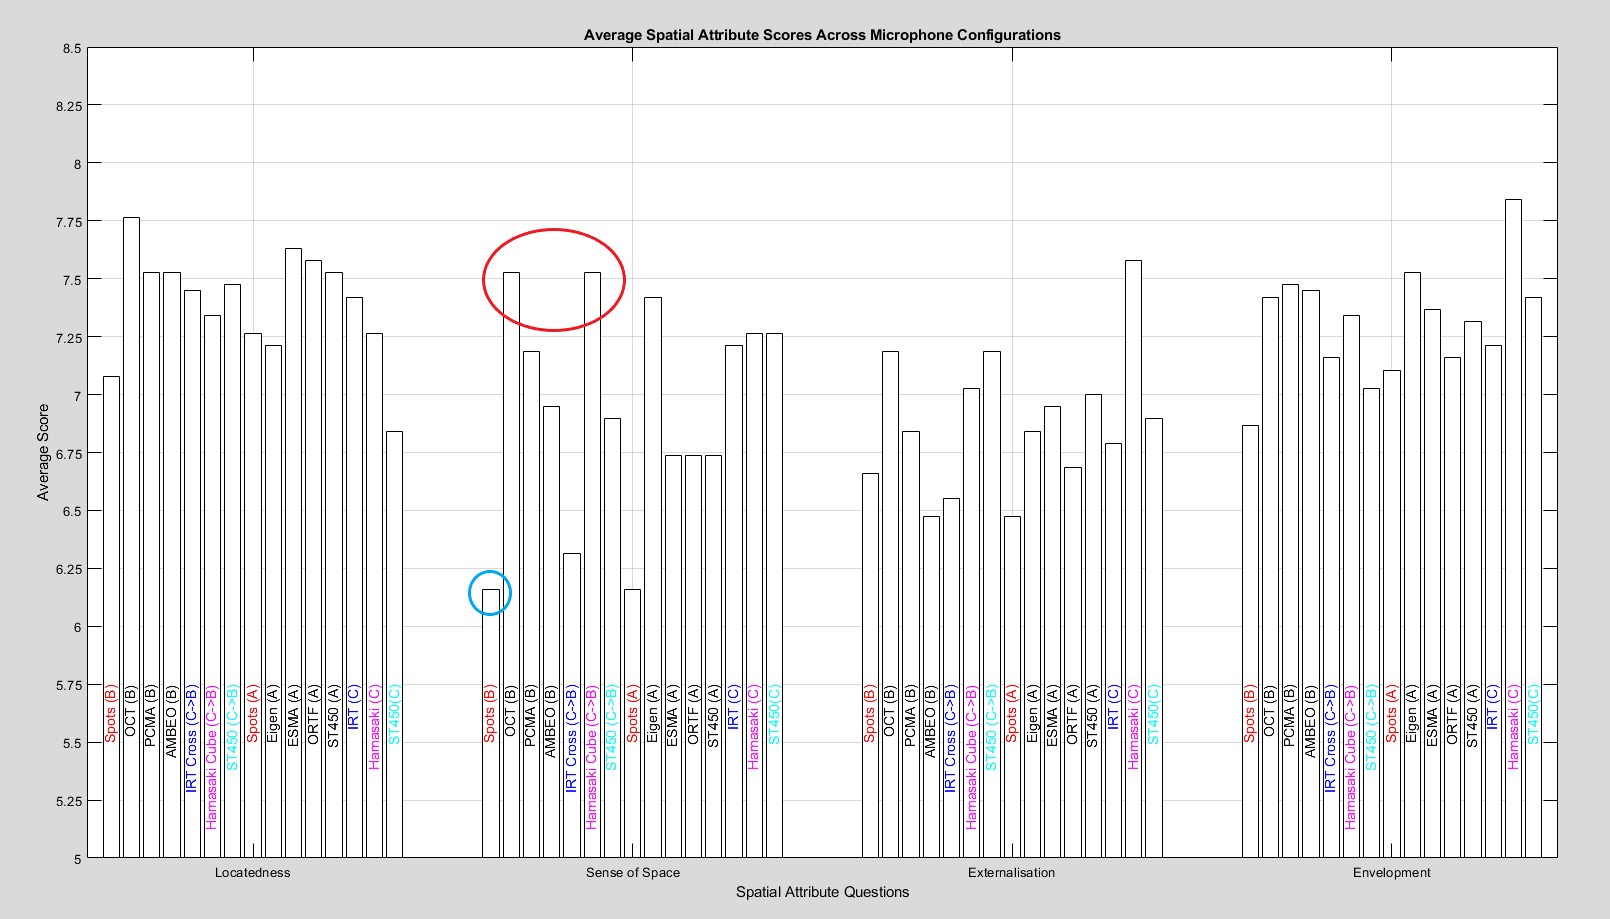
\includegraphics[width=0.5\textwidth]{images/plots/allMics_edit.PNG}
			\caption{Bar chart of the average SA score across all microphone configurations where (X) indicates the microphone location. The microphone names are displayed on their corresponding bar chart where (C->B) indicates a microphone from position C whilst viewing from B and (C) indicates a microphone from position C whilst viewing from position A}
			\label{image:sa_allmics} 
		\end{figure}

